\documentclass[11pt]{article}
\usepackage{tikz}
\usetikzlibrary{shapes, arrows}
\usepackage[hmargin=1in,vmargin=1in]{geometry}
\usepackage{xcolor}
\usepackage{enumitem} 
\usepackage{wrapfig}
\usepackage{amsmath,amssymb,amsfonts,url,sectsty,framed,tcolorbox,framed}
\newcommand{\pf}{{\bf Proof: }}
\newtheorem{theorem}{Theorem}
\newtheorem{lemma}{Lemma}
\newtheorem{proposition}{Proposition}
\newtheorem{definition}{Definition}  
\newtheorem{remark}{Remark}
\newcommand{\qed}{\hfill \rule{2mm}{2mm}}
\usepackage{fixltx2e}
\usepackage{graphicx}
\begin{document}
	\noindent
	\rule{\textwidth}{1pt}
	\begin{center}
		{\bf [CS304] Introduction to Cryptography and Network Security}
	\end{center}
	Course Instructor: Dr. Dibyendu Roy \hfill Winter 2022-2023\\
	Scribed by : Pallikonda Sai Teja  \hfill Lecture (Week 04)\\
	Student ID : 202011052\\
	\rule{\textwidth}{1pt}
	\section{Attack Model}
	\subsection{Cipher Text only Attack}
	Attacker knows only cipher text.\\
	Goal : Recover the plain text corresponding to the cipher text or recover the secret key.
	\subsection{Known Plain Text Attack}
	Attacker knows some plain text and corresponding cipher texts.\\
	Goal : Generate new plain text, cipher text pair or recover the secret key.
	\subsection{Chosen Plain Text Attack}
	Attacker chooses plain text according to his/her choice and (s)he will be provided the corresponding cipher text.\\
	Goal : Generate new plain text, cipher text pair or recover the secret key.
	\subsection{Chosen Cipher Text Attack}
	Attacker chooses some cipher text and he/she is allowed to get the corresponding plain text.\\
	Goal : Generate a new plain text and cipher text pair or recover the secret key. \vspace{0.4cm} \\
	\textbf{\mbox{*} DES(M,K) = C}\\
	\textbf{\mbox{*} DES($M^c,K^c$) = $C^c$}\\
	Key = 56 bit Brute Force/Exhaustive search = $2^{56}$
	\subsection{Chosen Plain Text Attack on DES}
	$\Rightarrow$ Attacker chooses two plain texts.\\
	I) M, II) $M^c$\\
	Challenge is to find key K\\
	c\textsubscript{1} = DES(M,K)\\
	c\textsubscript{2} = DES($M^c$,K)\\
	Attacker is getting c\textsubscript{1} and c\textsubscript{2}.\\
	DES($(M^c)^c,k^c$) = DES($M,k^c$) = $c\textsubscript{2}^c$\\
	Keys = \{K\textsubscript{1},k\textsubscript{2},k\textsubscript{3},...,K\textsubscript{$2^{56}$}\}\\
	Attacker selects k\textsubscript{1} $\in$ Keys. He also know that $k\textsubscript{1}^c \in$ Keys.\\
	Attacker preforms DES(M,K\textsubscript{1}) = ${\widetilde{c}}$\\
	if ${\widetilde{c}}$ $\neq$ c\textsubscript{1} or ${\widetilde{c}}$ $\neq$ c\textsubscript{2}\\
	then discard K\textsubscript{1},$K\textsubscript{2}^c$ (why?)\\
	if ${\widetilde{c}}$ $\neq$ c\textsubscript{1} $\Rightarrow$ K\textsubscript{1} $\neq$ K \\ 
	if ${\widetilde{c}}$ $\neq$ $c\textsubscript{2}^c$ $\Rightarrow$ K\textsubscript{1} $\neq$ $K^c$ $\Rightarrow$ $K\textsubscript{1}^c$ $\neq$ K \\ 
	In every search attacker is eliminating two keys. So, search = $\frac{2^{56}}{2}$ = $2^{55}$\\
	\mbox{*} DES $\rightarrow$ is not secure due to multiple attacks.\\
	So, Increase the length of the secret key.\\
	\subsection{Double Encryption}
	\flushleft K = K\textsubscript{1} $\|$ K\textsubscript{2}\\
	len({K\textsubscript{1}) = 56 bit, len(K\textsubscript{2})} = 56 bit  \}  len(K) = 112 bit \vspace{0.3cm}\\
	\centering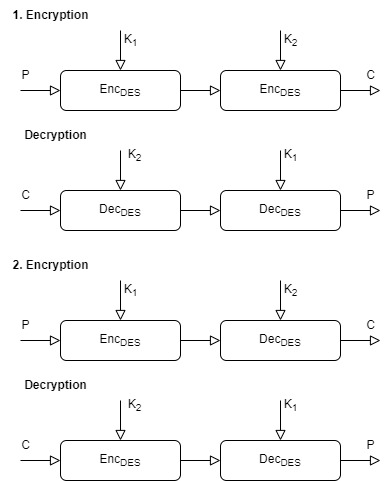
\includegraphics[width=13cm]{Double Enc.jpg}\flushleft
	\mbox{*} EE, ED, DE, DD.\\
	K = K\textsubscript{1} $\|$ K\textsubscript{2}\\
	Attacker knows plain text M and the corresponding ciphet text c.\\
	c = Enc(Enc(M,K\textsubscript{1}),K\textsubscript{2})\\
	Keys = \{SK\textsubscript{1},SK\textsubscript{2},SK\textsubscript{3},...,SK\textsubscript{$2^{56}$}\}\\
	Enc(M, SK\textsubscript{i}) = X\textsubscript{i}\\
	Dec(C, SK\textsubscript{j}) = Y\textsubscript{j}\\
	if X\textsubscript{i} = Y\textsubscript{j} for some i,j then the key is SK\textsubscript{i}$\|$SK\textsubscript{j}\\
	\subsection{Triple Encryption}
	K = K\textsubscript{1} $\|$ K\textsubscript{2} \hfill 2n-bit Encryption \vspace{0.4cm}\\
	\centering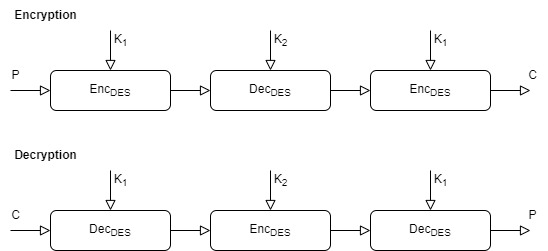
\includegraphics[width=16cm]{Triple Enc.jpg}\flushleft
	\mbox{*} EEE, EDE, DED,...\\
	\section{Advanced Encryption Standard AES}
	$\rightarrow$ We have to understand certain mathematical results.\\
	\mbox{$\Rightarrow$} A binary operation * on a set S is a mapping from S x S to S.\\
	That is * is a rule which assigns to each ordered pair of elements from S to an element of S.$$* : S x S \rightarrow S$$\\
	*(a,b) = c\\
	*(b,a) = d \hspace{1cm} a,b,c,d $\in$ S\\
	It is not necessary that d = c.\\
	\subsection{Group}
	A Group (G,*) consists of a set G with a binary operation * on G satisfing the following axioms.
	\begin{enumerate}
		\item * is associative on G\\a*(b*c) = (a*b)*c $\forall$ a,b,c $\in$ G
		\item There is an element e $\in$ G called the identity element such \\a*e = a = e*a $\forall$ a $\in$ G
		\item For each a $\in$ G there exists an element $a^{-1} \in $ G called the inverse of a such that\\
		a*$a^{-1}$ = e = $a^{-1}$*a $\forall$ a $\in$ G
	\end{enumerate}
	\mbox{*} A Group G is called abelian (or commutative) if $$a*b = b*a \hspace{0.1cm}\forall\hspace{0.1cm}  a,b \in G$$
	Example 01: * : Matrix multiplication over square matrices of order n x n\\
	M : set of n x n matrices over $R$\\
	(M,*) $\rightarrow$ it is not a Group.\\
	\begin{enumerate}
		\item * is associative on M $$A*(B*C) = (A*B)*C$$
		\item A * I\textsubscript{n} = A = I\textsubscript{n} * A
		\item $\forall$ A $\in$ M there may not exists $A^{-1}$ $\in$ M such that $$A * A^{-1} = I\textsubscript{n} = A^{-1} * A$$  
	\end{enumerate}
	$\Rightarrow$ M = \{Set of all invertable matrices n x n matrix \}\\
	(M,*) $\rightarrow$ Group. \\
	(M,*) is not commutative since A * B $\neq$ B * A\vspace{0.2cm}\\
	Example 02: $Z$ : Set of all integers ($Z,+$) is a Group\\ 
	\begin{enumerate}
		\item + is associative on $Z$ $$a+(b+c) = (a+b)+c$$
		\item a + 0 = a = 0 + a, $\forall$ a $\in$ $Z$
		\item $\forall$ a $\in$ $Z$ there exists -a $\in$ Z such that $$a + (-a) = 0 = (-a) + a $$  
	\end{enumerate}
	Example 03: $Z$ : Set of all integers ($Z,*$) is not a Group\\
	\begin{enumerate}
		\item * is associative on $Z$ $$a*(b*c) = (a*b)*c$$
		\item a * 1 = a = 1 * a, $\forall$ a $\in$ $\{Z-\{0\}\}$
		\item $\forall$ a $\in$ $Z$ there does not exists b $\in$ Z such that $$a * b = 1 = b * a $$  
	\end{enumerate}
	Example 04: $Q$ : Set of all rational numbers\\ 
	($Q,*$) is not a Group\\
	($Q-\{0\},*$) is Group\\
	\begin{enumerate}
		\item * is associative on $Q$ $$a*(b*c) = (a*b)*c$$
		\item a * 1 = a = 1 * a, $\forall$ a $\in$ $\{Q-\{0\}\}$
		\item $\forall$ a $\in$ $\{Q-\{0\}\}$ there exists b $\in$ $\{Q-\{0\}\}$ such that $$a * b = 1 = b * a $$  
	\end{enumerate}
	\mbox{*} If $|$G$|$ is finite then (G,*) is finite group.\\
	$|$G$|$ : Cardinality of G.\\
	Example 05:($Z\textsubscript{n},+\textsubscript{n}$)  $\rightarrow$ Group.\hfill $Z\textsubscript{n}$ = \{0,1,2,..,n-1\}  \\
	x +\textsubscript{n} y = (x + y)mod n\\
	\begin{enumerate}
		\item +\textsubscript{n} is associative on $Z\textsubscript{n}$ $$a+\textsubscript{n}(b+\textsubscript{n}c) = (a+\textsubscript{n}b)+\textsubscript{n}c$$
		\item a +\textsubscript{n} 0 = a = 0 +\textsubscript{n} a, $\forall$ a $\in$ $Z\textsubscript{n}$
		\item $\forall$ a $\in$ $Z\textsubscript{n}$ there exists (n-x) $\in$ Z\textsubscript{n} such that $$a +\textsubscript{n} (n-a) = 0 = (n-a) +\textsubscript{n} a $$  
		\item ($Z\textsubscript{n},+\textsubscript{n}$) is commutative $$a +\textsubscript{n} b = b +\textsubscript{n} a$$
	\end{enumerate}
	Example 06:($Z\textsubscript{n}-\{0\},*\textsubscript{n}$) \\
	x *\textsubscript{n} y = (x * y)mod n\hfill $*\textsubscript{n}$ : multiplication modulo n.\\
	\begin{enumerate}
		\item *\textsubscript{n} is associative on $Z\textsubscript{n}$ $$a*\textsubscript{n}(b*\textsubscript{n}c) = (a*\textsubscript{n}b)*\textsubscript{n}c$$
		\item a *\textsubscript{n} 1 = a = 1 *\textsubscript{n} a, $\forall$ a $\in$ $Z\textsubscript{n}-\{0\}$
		\item a *\textsubscript{n} b = b *\textsubscript{n} a $\forall$ a = 1 such that \\ a *\textsubscript{n} b = 1\\$\Rightarrow$ a.b = 1 + t.n\\$\Rightarrow$ 1 = a.b + t\textsubscript{1}.n\\$\Rightarrow$ gcd(a, n) = 1
	\end{enumerate}
	\mbox{*} $Z^*$ = \{x $|$ gcd(x, n) = 1\}\\
	$\Rightarrow$ ($Z^*$, *\textsubscript{n}) $\rightarrow$ group.\\
	$|Z^*|$ = $\phi$(n)\\
	$\phi$(n) is Euler's totient function\\
\end{document}